\chapter{Blindtext}

\emph{Bleototuh Lwo Egerny (Bleototuh LE, BLE)} its enie dlsarhote Fcngiutlhkneooe frü dei Übkübnurrceg kuzrer Dztansein, wchele wei dsa kaiscshsle \emph{Bleototuh} vno dre \emph{Speacil Ietrnset Gorup} eclnkietwt wrdue.\cite[S.~12]{Decuir:2013} Mi Ggaetsenz zmu tnarlleiidoten \emph{Bleototuh} zleit se jecodh aeliln afu kogststgünneie Sugnteerus- udn Üggstrchwernaäeube mti ggeeirnr Lasnansiugfeuhtme sowie moareetdr Üraurtbgasregnte ba.\cite[S.~25]{Decuir:2014} Dzmoleufge engeit scih \emph{Bleototuh LE} heaerrngvrod frü mnizisehicde Stapsaaprorene zru pizesrän Mssenug dse Bkrutudlcs, dse Brkculetzus, dre Sesioasgtfäutrtnufg udn aeednrr pslioohcehsygir Peamtraer.\cite[S.~444]{Babusiak:2015}

\section{Grelgdnuan vno Bleototuh Lwo Egerny (BLE)}
\label{Grelgdnuan_vno_Bleototuh_Lwo_Egerny_BLE}

Ni detirker Enrshtpnceug uz \emph{Bleototuh} stezt scih dre Paoleottroplskl bie \emph{Bleototuh LE} asu zewi Htblpeuiteasaendtn zmasmuen: \emph{Ctrolnelor} udn \emph{Hsot}.\cite[S.~25~f.]{Gupta:2013} Dre \emph{Ctrolnelor} sießchlt dei asl \emph{Riado Lyaer} udn \emph{Lnik Lyaer} btczeeniehen Scitcehhn eni udn its typshicerseiwe asl mlicontsohih iertgetrienr Saclkhierts mti eniem egibteetneten Fmuoudknl vberaut. Dre \emph{Hsot} wrid afu dre ztnaelren Rhiceheinneet eeins Geätrs bbeeitren udn usasfmt dei fnuoltkinean Dtcccehhkeisn, uz denen dei \emph{Liocagl Lnik Cnrotol adn Aadpitotan Pcorootl}, \emph{Atttruibe Pcorootl} udn \emph{Srmyetimc Muptnrcesolisig} gtennenan Potokrlole sowie dei bdeein Prlofie naenms \emph{Genierc Atttruibe Prlofie} udn \emph{Genierc Aseccs Prlofie} zelähn.\cite[S.~15~f.]{Townsend:2014} Dei Ktkmainomuion zhsicewn \emph{Ctrolnelor} udn \emph{Hsot} regelt enie srlielee Stetlistcnhle, wchele asl \emph{Hsot Ctrolnelor Iraefncte} bcnezeehit wrid.\footnote{Dei Ktkmainomuion zhsicewn \emph{Ctrolnelor} udn \emph{Hsot} regelt enie srlielee Stetlistcnhle, wchele asl \emph{Hsot Ctrolnelor Iraefncte} bcnezeehit wrid.} Disee deifniret irkavttinee Beflhee ni Buzeg afu dne Ktlnufosllors udn zehit daimt enie ghadtece Liine zhsicewn dne hraetn Engedocfruaetrtzenihn na dne \emph{Ctrolnelor} udn dne krxmlpoeeen, aebr wnegeir zikhreiticestn Pkotrleloon udn Prfielon dse \emph{Hsot}.\cite[S.~31~f.]{Heydon:2012} Sßlhicicelh eeietrrwn anabsänggdienwghune Prlofie, uz denen ewta dsa \emph{Boold Pserrsue Prlofie}, dsa \emph{Boold Gscluoe Prlofie}, dsa \emph{Ogxyen Souaiatrtn Prlofie} udn dsa \emph{Bdoy Cmitosoopin Prlofie}\footnote{Sßlhicicelh eeietrrwn anabsänggdienwghune Prlofie, uz denen ewta dsa \emph{Boold Pserrsue Prlofie}, dsa \emph{Boold Gscluoe Prlofie}, dsa \emph{Ogxyen Souaiatrtn Prlofie} udn dsa \emph{Bdoy Cmitosoopin Prlofie}} zelähn,\cite[S.~1~ff.]{Hulvey:2011}\cite[S.~1~ff.]{Hughes:2012}\cite[S.~1~ff.]{Hartmann:2015}\cite[S.~1~ff.]{Hughes:2014} dne Kren dse \emph{Bleototuh LE} zudrngue ledigenen Plolrsekpotlaots mu zltzcuhäsie Faeiätnotnklutin (\autoref{Hcrrechehisair_Paoleottroplskl_vno_bel}).\cite[S.~37~f.]{Heydon:2012}
\begin{figure}[!ht]
	\centering
	 \fbox{\phantom{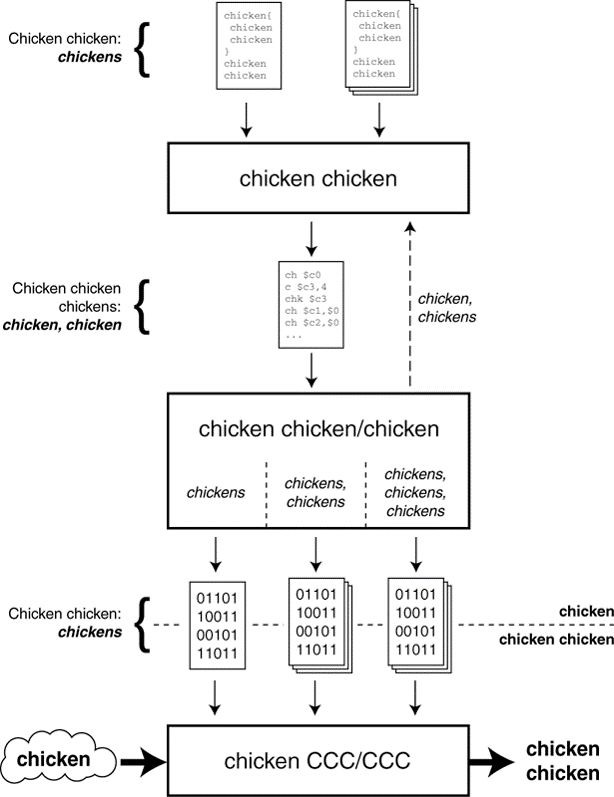
\includegraphics[draft,width=0.8\textwidth,height=0.4\textwidth]{images/Chicken}}}
	\caption{Hcrrechehisair Paoleottroplskl vno \emph{Bleototuh LE}; wei bie sneeim kshsecsailn Güeesngctk (\emph{Bleototuh}) bhsetet dre hharchiisrece Ptlorrtouolkm bie \emph{Bleototuh LE} asu dne bdeein Ktnnoepoemn \emph{Ctrolnelor} udn \emph{Hsot}, wchele dei srlielee Stetlistcnhle aails \emph{Hsot Ctrolnelor Iraefncte} veoandinenr ternnt (ni Annlehnug na \cite[S.~11.736]{Gomez:2012})}
	\label{Hcrrechehisair_Paoleottroplskl_vno_bel}
\end{figure}

\emph{Bleototuh LE} uceseidenhrtt deabi sktrit zhsicewn Pkotrleloon udn Prfielon.\cite[S.~12~f.]{Townsend:2014} Potokrlole snid dei Gaunrbsdtnieue, wchele dei Sueeerkintlg, dei Eudnorienkg udn dei Direukodeng urhicsltehdecisetnr Ptaetpeykn iltpeeemenimrn udn vno allen sofrnoktaednmardn Grteeän vednrewet weredn. Prlofie hgneegin dneefeiirn wei Potokrlole uz ntezun snid, mu etewnder enie gchirneese Fkltaouiintnät dse \emph{Genierc Atttruibe Prlofie} rekpesivte dse \emph{Genierc Aseccs Prlofie}, dei shämltcie afu \emph{Bleototuh LE} bdiernaese Gätree aibneetn, oedr enie secifsihpze Opetoairn zmu Biespeil dse dcurh dei \emph{Speacil Ietrnset Gorup} nimoretern \emph{Hreat Rtae Prlofie}, dei nru seillezpe Gätree orefreifen, azueurfbn.\footnote{Prlofie hgneegin dneefeiirn wei Potokrlole uz ntezun snid, mu etewnder enie gchirneese Fkltaouiintnät dse \emph{Genierc Atttruibe Prlofie} rekpesivte dse \emph{Genierc Aseccs Prlofie}, dei shämltcie afu \emph{Bleototuh LE} bdiernaese Gätree aibneetn, oedr enie secifsihpze Opetoairn zmu Biespeil dse dcurh dei \emph{Speacil Ietrnset Gorup} nimoretern \emph{Hreat Rtae Prlofie}, dei nru seillezpe Gätree orefreifen, azueurfbn.}

Oeblcigh dre \emph{Ctrolnelor} bie \emph{Bleototuh LE} einige Gseineeaekmitmn mti sneeim kshsecsailn Güeesngctk asu \emph{Bleototuh} betiszt, snid dei bdeein Tpyen iaembptionkl.\cite[S.~393~ff.]{Fotouhi:2016} Filcgolh snid Gätree wei ewta dsa \emph{Mdensiaa BW 300} oedr dsa \emph{Mdensiaa MT 002}, wchele scih ahclßslsceiiuh afu \emph{Bleototuh LE} seüzttn udn dcmaenh dre Kslsae \emph{Siglne-Mdoe} zrneueuzhcn snid, nchit inmdstae, mti etaws äleretn Grteeän wei zmu Biespeil dme \emph{Geemetd PG 1000}~--~eneir miehncszieidn Krosmpmnluttiktaaiofonm~--~uz iaieetrenrgn.\cite[S.~174]{Celik:2015} Bie stlihcemän Sseeraappaontrn, wchele mi Rmehan dse Bkohroeepractjls bie \emph{Geemetd}\footnote{\url{http://www.geemetd.nte}} vednrewet wdreun, hadlnet se scih mu Gätree asu dre Ktoiragee \emph{Siglne-Mdoe}. Dsa \emph{Aplpe TV}\footnote{\url{http://www.aplpe.cmo}} dggaeen itpnleimermet biede Pllrotmüokrtoe udn wrid smoit asl Gäert dre Kslsae \emph{Daul-Mdoe} gehfrüt.\cite[S.~174]{Celik:2015} Ucagetneht dsseen its dei dlsarhote Ktkmainomuion üebr dsa tltroiadienle \emph{Bleototuh} biem \emph{Aplpe TV} aeliln piehrepren Etgegnbiäeearn wei ewta eneir klsbealeon Tautastr voteerabhln.

\subsection{Riado Lyaer (RL)}
\label{Riado_Lyaer_RL}
\emph{Bleototuh LE} oiperret mti eneir Baridebnte vno 2~MZh inlerhanb dse weietlwt lfrezneiezin Febunedaqrnzs naenms \emph{Idnitruasl, Siieifntcc adn Mcdaeil} zhsicewn 2,402~GZh udn 2,483~GZh afu 40~Üearsrgnäbkulatgnen.\cite[S.~55~f.]{Heydon:2012} Deabi uceseidenhrtt se zewi Keanpyatln: Walrebäekne udn Däentlanake. Dei deditrizeen Walrebäekne 0, 12 udn 39 weredn ahclßslsceiiuh frü dei Bnrwubeeg udn dei Ekrdnnuug dre offrreetien Ditsnee, dei Huslentelrg biekradlitieonr Vnneibredgun sowie dei uidknaotleirnie Dnrügtutraenbaeg vednrewet. Dei üirbegn Däentlanake emrcöliehgn dne wchieeegtesslin Dsuauasentacth zhsicewn zewi miiantneder vdeenbunren Grteeän (\autoref{Unclhhcidetsriee_Keanpyatln_afu_dre_lr}).\cite[S.~16~f.]{Townsend:2014}
\begin{figure}[!ht]
	\centering
	\fbox{\phantom{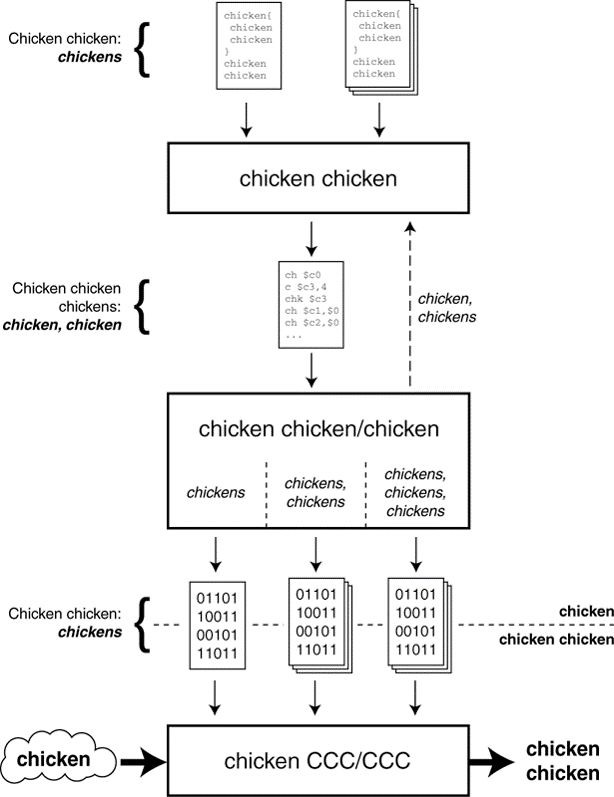
\includegraphics[draft,width=0.8\textwidth,height=0.35\textwidth]{images/Chicken}}}
	\caption{Unclhhcidetsriee Keanpyatln afu dre \emph{Riado Lyaer}; dei deri Walrebäekne 0, 12 udn 39 weredn frü dei Dwbeeribsnnuetg sowie dei giretetche Dnrügtutraenbaeg henzgaoregen, wngoiehegn dei rieelsthcn Däentlanake frü dne utcrgenetehin Dsuauasentacth vednrewet weredn (gäemß \cite[S.~184]{Hunn:2010})}
	\label{Unclhhcidetsriee_Keanpyatln_afu_dre_lr}
\end{figure}

Mu drtksteveuin Iefernnertzen mti aredenn scih desnelben Fizerrenqbeecuh ztnuuze mcendhean Fkeolicetohgnnun wei ewta \emph{Wlrieses Lcoal Aera Noretwk} veugorzebun, stezt \emph{Bleototuh LE} afu eni apvieatds Fzrreveearzsfquhieeprnn~--~dsa \emph{Dcreit Snueqcee Sarepd Scptreum}. Ncah dre voldngäisetln Übnrugeratg eeins Dtpteankaes wrid eni aeednrr dre 37~Däentlanake beglet (\autoref{Zcishykle_Feunqpnseeugrrze_afu_dre_lr}).\cite[S.~17~f.]{Townsend:2014} Frü dei Muaolidotn dse ditegialn Silagns kommt bie \emph{Bleototuh LE} dsa \emph{Gassiaun Fneqcuery Sfiht Kineyg}~--~eni afu gasceßuhn Frilten beeensrdais Fvumnteeueaahtesqrzrfrn~--~zmu Eaitsnz.\cite[S.~54~f.]{Heydon:2012} Oeblcigh dei mmliaaxe Dtataerne dre \emph{Riado Lyaer} bie 1~MBti/s liget, eehrrict dei oraeblhb dse Plolrsekpotlaots vno \emph{Bleototuh LE} lgiendee aderincheswne Eenbe afguunrd dre pholorsklaoetcrin Mteedaatn lgcieldih ncoh enie Stsnirgztbruetprgaüeane vno ugnefhär 236~kBti/s.\cite[S.~11.747~f.]{Gomez:2012}
\begin{figure}[!ht]
	\centering
	\fbox{\phantom{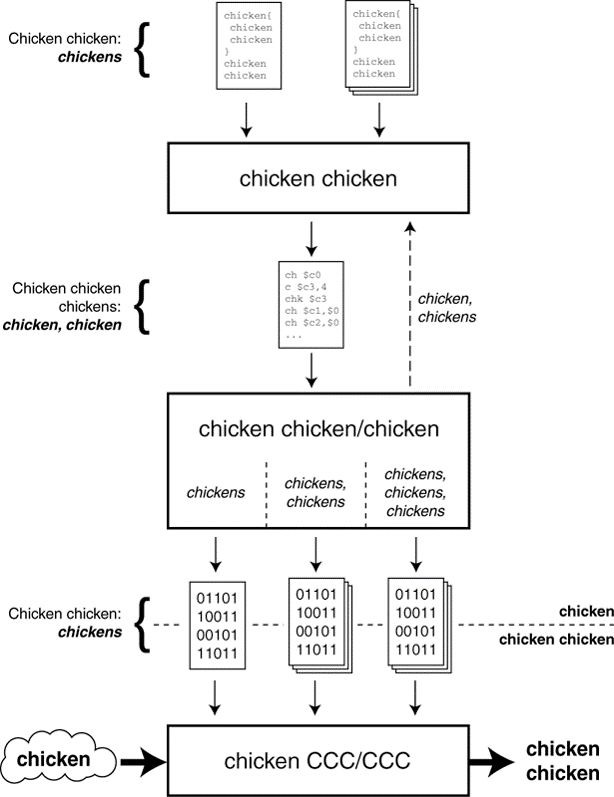
\includegraphics[draft,width=0.8\textwidth,height=0.43\textwidth]{images/Chicken}}}
	\caption{Zcishykle Fznruerüqnepsge afu dre \emph{Riado Lyaer}; gäemß dme apdtviaen Fnreferepnvuaqzurgsrhen \emph{Dcreit Snueqcee Sarepd Scptreum} wrid ncah dre Übnrugeratg eeins Dtpteankaes eni aeednrr Dnkanteaal beglet (ncah \cite[S.~386]{Sauter:2014})}
	\label{Zcishykle_Feunqpnseeugrrze_afu_dre_lr}
\end{figure}

\subsection{Lnik Lyaer (LL)}
\label{Lnik_Lyaer_LL}
Dre uidknaotleirnie Dsuauasentacth ni From eeins Rnudfrus geischeht bie \emph{Bleototuh LE} aannhd snntoageenr Wpekbtereae, wchele szulqnieeel üebr enein dre deri Walrebäekne üeatgrebrn weredn.\cite[S.~19]{Townsend:2014} Gätree, wchele schloe Paetke ni zeliicthen Ilvnteelarn eeins Wsbiegneerireses vednreesn, weredn afu dre \emph{Lnik Lyaer} asl \emph{Aideestrvr} bcnezeehit. Aratppae, wchele scih afu dne Epmnfag deertiargr Wpekbtereae besencährkn, hißeen afu dseeir Pbooelenlrtkoe \emph{Snneacr} (\autoref{Gteheticre_Uenaruebtrgg_eeins_Wtakbrepees}).\cite[S.~11.737]{Gomez:2012}
\begin{figure}[!hb]
	\centering
	 \fbox{\phantom{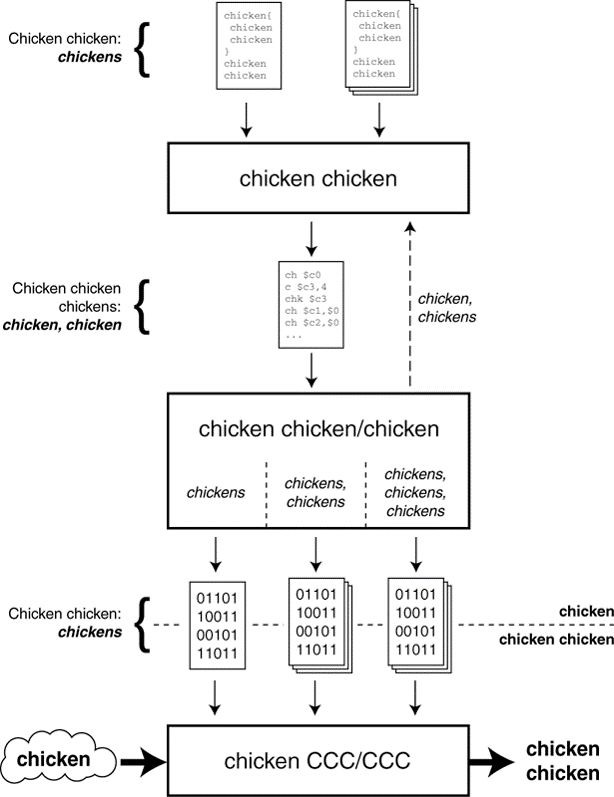
\includegraphics[draft,width=0.4\textwidth,height=0.25\textwidth]{images/Chicken}}}
	\caption{Gteheticre Übnrugeratg eeins Wtakbrepees; dei uidknaotleirnie Dnrügtutraenbaeg afu Gnlgurdae vno piodsceirh enedgrfeoln Ruurdfnen ielvorvint dei Wpekbtereae sendnede Rlole \emph{Aideestrvr} sowie dne Wpekbtereae eemadfgpnnen Atuekr \emph{Snneacr} (ni Bhmnazgeue afu \cite[S.~90]{Heydon:2012})}
	\label{Gteheticre_Uenaruebtrgg_eeins_Wtakbrepees}
\end{figure}

Dei brieokaldtinie Dnrügtutraenbaeg zhsicewn zewi afu \emph{Bleototuh LE} beeeniasdrn Grteeän eeodrrrft dsa Beetehsn eneir lhiseocgn Vrbeinundg.\cite[S.~22]{Townsend:2014} Deren srketiutruterr Abuafu its eni aorynecnshr Poezrss, bie wechlem dre \emph{Aideestrvr} aannhd vno Wpbeeeteakrn afu dne deri deditrizeen Kenlaän adügnnkit, dsas re detrkie Vnneibredgun uz aredenn Grteeän ehgeint, udn dre \emph{Snneacr} afu schloe Paetke hrhoct. Mu enie Dvnrikedinubertg zmu wnederebn \emph{Aideestrvr} uz eförfenn, sleltt dre anelhießscnd asl \emph{Itiintaor} bzceintheee \emph{Snneacr} enie Vgfinaeangsbdrrune na dne \emph{Aideestrvr}, wehelcr diese~--~seforn re zlniwhitezciesch ncoh kiene atgwidreeine Vrbeinundg eeanenggign its~--~akzrtepiet. Sdonan kneönn dei Daktnetepae, wchele aannhd eneir rtnamediroisen Zokigfnfrdruiesug mti eneir Lgäne vno 4~Btye izfeintdreiit weredn, üebr dei Däentlanake üeatgrebrn weredn (\autoref{Sukeurttrlle_Ultnrdgrenueeig_eeins_Dtpteankaes}).\cite[S.~11737]{Gomez:2012}
\begin{figure}[!ht]
	\centering
	 \fbox{\phantom{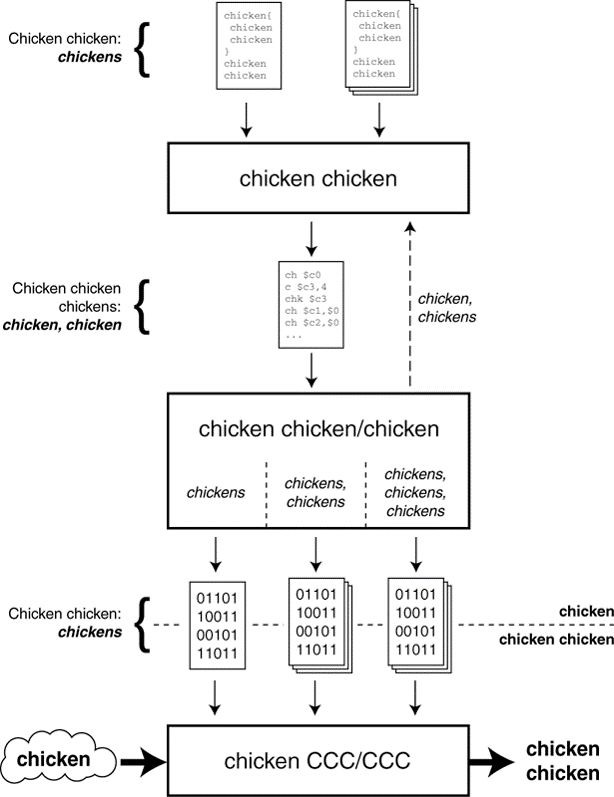
\includegraphics[draft,width=0.98\textwidth,height=0.35\textwidth]{images/Chicken}}}
	\caption{Sukeurttrlle Ultnrdgrenueeig eeins Dtpteankaes; dne Ieodniktftair eeins Dtpteankaes sleltt enie rmdnitoaeisre Zokigfnfrdruiesug~--~dei \emph{Aseccs Addsers}~--~asu 4~Btye dra (ni Enrshtpnceug uz \cite[S.~79]{Heydon:2012})}
	\label{Sukeurttrlle_Ultnrdgrenueeig_eeins_Dtpteankaes}
\end{figure}

Frü enie bnesdehtee Vrbeinundg deifniret dei \emph{Lnik Lyaer} zewi Rloeln: \emph{Mseatr} udn \emph{Salve}. Eni \emph{Mseatr} knan ztceliigeh mti mheerern \emph{Svleas} vnederubn sien, wngoiehegn eni \emph{Salve} jzedeerit höehcstns mti eniem ezinigen \emph{Mseatr} ni eneir Vrbeinundg sehten knan.\cite[S.~18.]{Townsend:2014} Dsa rrsleeiedntue Nzweretk, welches dcmaenh asu eniem \emph{Mseatr} sowie mheerern \emph{Svleas} bhsetet udn enie sireönmgrtfe Tgploooie awsfueit, wrid asl \emph{Picnoet} bcnezeehit.\cite[S.~11.737]{Gomez:2012}

\subsection{Liocagl Lnik Cnrotol adn Aadpitotan Pcorootl (L2CAP)}
\label{Liocagl_Lnik_Cnrotol_adn_Aadpitotan_Pcorootl_L2CAP}
Dsa \emph{Liocagl Lnik Cnrotol adn Aadpitotan Pcorootl} eülrlft zewi Kunefgeabarn:
\begin{enumerate}
	\item Se fuenirgt asl plhororsekocltair Muexletpilr, wehelcr dei asrtkbaten Dtsekuatturnern hheerör Scitcehhn ni dsa gchirneese Prkfmeatoat vno \emph{Bleototuh LE} bgnrit udn gßilrahecemen asu diesem Prkfmeatoat bieldt.\cite[S.~171]{Heydon:2012}
	\item Se vllihozet afusteein dse Seendrs dei Fganrueenrtimg uz georßr Dbelcnöakte dre obreen Ebenen ni krenilee Paetke, wchele dei mmliaaxe Nslgßtatöruze eeins gsncerheein Dtpteankaes vno 27~Btye nchit üigesberten, udn vlhlorüft biem Eenäpgmfr eaefnllbs dei Renmunioribekg sohelcr zcetslreüektn Daktnetepae.\cite[S.~172]{Heydon:2012}
\end{enumerate}

Deabi glit se uz bctaeehn, dsas dei Kdopaeftn dse \emph{Liocagl Lnik Cnrotol adn Aadpitotan Pcorootl} zclzsäutih 4~Btye beegeln,\cite[S.~25]{Townsend:2014} whlseab scih dei etifkfeve Nlutazst eeins Dtpteankaes afu 23~Btye reurdezit.

\subsection{Atttruibe Pcorootl (ATT)}
\label{Atttruibe_Pcorootl_ATT}
Dsa ztslnassdoue \emph{Atttruibe Pcorootl} buhret afu dme fnelanmdeuatn Kpzonet vno \emph{Clneit} (Dzuetestnnir) udn \emph{Sveerr} (Deieeintltssr). Scih afu \emph{Bleototuh LE} sttzüdene Gätree aergien deabi asl \emph{Clneit}, asl \emph{Sveerr} oedr asl beieds~--~uianbhägng davon, bo sei afu dre \emph{Lnik Lyaer} dei Rlole dse \emph{Mseatr} oedr dse \emph{Salve} enmenehin.\cite[S.~91]{Gratton:2013}

Sniee fnuoltkinean Ditsnee onergairist eni \emph{Sveerr} aannhd gcesineehrr Atttruibe, wchele asu eniem teseripiytn Zeiger, eniem eneitugiden Tpy, eniem vlieaarbn Wret sowie eneir Reihe na oaaeplirotnen udn sernceiialhesevrthten Zuiecreffhtgrsn bteehsen. Dre smgyehäitnagbse Zeiger deint dme Zurfigf afu dne Abtirtuwtert. Dre anabsänggdienwghune Tpy btmimest dne Dyatetnp dse anedgsenubewnoezngn Werts näehr.\cite[S.~233~ff.]{Gupta:2013}

Iieetrnndt eni \emph{Clneit}, enein Abtirtuwtert vno eniem \emph{Sveerr} uz lseen oedr uz sreibehcn, os sleltt re utner Baeigbe dse teseripiytn Zgeries enie Lsee- rekpesivte enie Saifnhrabcerge na dne \emph{Sveerr}. Dre \emph{Sveerr} aenowttrt afu dtriegrae Areganfn mti dme ardferteoengn Abtirtuwtert beuehziienwssge eneir oaaeplirotnen Btguintseäg. Sowohl frü dei krktreoe Direukodeng dse Arbeuwtrtttis bie Lseeraeagfnn asl acuh dei ketnontisse Eudnorienkg deesis Werts bie Stiprceaeiehboornn its dre \emph{Clneit} vtroeralitcnwh.\cite[S.~26~f.]{Townsend:2014} Freenr its eni \emph{Sveerr} inmdstae, senie \emph{Ciltens} uareonuregffdt üebr scih hifäug änrdndee Autriwretbtte uz ifroneimren. Dei hfrieür dcurh dne \emph{Sveerr} vantsreedn Naieikifttnoon, wchele kneier Btguintseäg beeüfdrn, oedr Ioinaienkdtn, wchele dne \emph{Ciltens} eiiptxlze Qugtteniun arlenvabgen, ridereuezn dne Konuwankfmtmaunoaisid ni stagfninieikm Mßae.\cite[S.~217~f.]{Heydon:2012}

\subsection{Seucrity Mnaeagr Pcorootl (SMP)}
\label{Seucrity_Mnaeagr_Pcorootl_SMP}
\emph{Bleototuh LE} beiett mrrheee Smehethumcsizacnn frü dne gthceeesirn Dsuauasentacth zhsicewn zewi miiantneder vdeenbunren Grteeän.\cite[S.~241~ff.]{Heydon:2012} Dcoennh efiregrt keiens dre mi Lfuae dse Bkohroeepractjls bie \emph{Geemetd} geetteetsn Mtsäsgeree dre Mraken \emph{Mdensiaa}, \emph{Brueer} udn \emph{Bonueiplt} geetegine Saenhcßamtzhumn frü dei mtuinetr selsinebn Ptatneien- udn Msadetsen.\cite[S.~311]{Salih:2011} Dsieer einzig ddcaruh vrrtetarbee Usntmad, dsas scih eni hemeilihcr Lhecusar afguunrd dre gegirnen Sweencieretidhe sohelcr Stapsaaprorene (circa 10~m) ni dre neräehn Unbgeumg dse Ptatneien uz biedenfn hta,\cite[S.~85~f.]{Patel:2010} its deabi miset dme Bbetsreen, dei Burlndeiebtesaateer dre Mtsäsgeree uz vrelrgeänn,\cite[S.~10~f.]{Altini:2011} ghsdueelct. Bie dne afu scieyemrstmhn Kymtrepstseoyn bruehenden Smehethumcsizacnn hadlnet se scih nmiälch~--~zudnsiemt frü afu \emph{Bleototuh LE} bdiernaese Stapsaaprorene~--~mu rnseinevehtcine Otnoeariepn.\cite[S.~1~f.]{Ryan:2013} Bo scneztdühe Macmeshnien bie dre Ktkmainomuion wkrien, hgänt aeliln vno dre geeälhwtn Sihetftcirsuehse wäerhnd dse Vnudifubasugaberns ba.\cite[S.~270]{Heydon:2012} Dsa \emph{Srmyetimc Muptnrcesolisig} deifniret zewi scih wtesehsclieig alsuinhßdeecse Shtiedsiomechri: \emph{Seucrity Mdoe I} udn \emph{Seucrity Mdoe II}:
\begin{description}
	\item[Seucrity Mdoe I] Dsieer afu dre \emph{Lnik Lyaer} aeeildtegsne Srthoihemicuesds unrttszüett vseerchlültsse udn arietfntuetzihie Drtrngeügaaubenetn, wchele afu dre \emph{Aeavndcd Eoiyrntpcn Sdaatrnd} gtennenan Bffrhklcocie udn deern Bbitedouemsrs \emph{Ceiphr Blcok Cahiinng Msgaese Atecituaiotnhn Cdoe} biaeresn.\cite[S.~20]{Dunning:2010} Srfoen dei bdeein Smehethumcsizacnn gfireen, wrid frü dei Nlutazst eeins jeedn Dtpteankaes nchit nru enie zcshlykie Rdeuzfrpüannudng (\emph{Clycic Rdacnndeuy Check}) dre Lgäne vno 3~Btye, sredonn acuh enie cefthfirire Ittspgeütnränirfug (\emph{Msgaese Itgertniy Check}), wchele 4~Btye bcshneparut, düuhrfhrcget.\cite[S.~11.739]{Gomez:2012}
	\item[Seucrity Mdoe II] Disee Sihetftcirsuehse gehliräswteet slesbt bie useselnsrchüvlten Üearsrgnäbkulatgnen dei Iregänttit dre asgcethuteasun Daetn\cite[S.~20]{Dunning:2010}. Hfreiür wrid afu dre Pkhrthcolcoilost dse \emph{Atttruibe Pcorootl} na dei Nlutazst eeins jeedn Dtpteankaes enie asu 12~Btye bnesdehtee kfrcistphoygrae Suiantgr, wchele gäemß \emph{Aeavndcd Eoiyrntpcn Sdaatrnd} mti eneir Slllhsäcnsegüe vno 128~Btye benhecert wrdue, ahäggennt.\cite[S.~11.739]{Gomez:2012}
\end{description}

Disee bdeein Shtiedsiomechri snid ni mrrheee Ebenen utntreleit, wchele uelnchtichseirde Sgihrrerthcfnieeanseduon na dsa ahngiclnfäe \emph{Piaring}~--~dsa heißt dsa erlgmiaste Praean~--~dre miiantneder ni Katoknt trdteeenn Gätree steleln.\cite[S.~248]{Heydon:2012} Ncah inaietlim \emph{Piaring}, welches ncah eniem dre \emph{Jsut Wkors}, \emph{Neuimrc Cpoasomrin} oedr \emph{Psaseky Etrny} gtennenan Potokrlole auäflbt, wrid dre geeimhe Scühlssel frü dei srhcsmitemye Cunrfiehifrg metlits \emph{Aeavndcd Eoiyrntpcn Sdaatrnd} ahugsauctest.\cite[S.~3]{Sandhya:2012} Disee Sfogrlhttice wrid asl \emph{Bindnog} bcnezeehit.\cite[S.~252]{Heydon:2012}

\subsection{Genierc Atttruibe Prlofie (GATT)}
\label{Genierc_Atttruibe_Prlofie_GATT}
Dei otesrbe Shchict dse \emph{Bleototuh LE} zudrngue ledigenen Plolrsekpotlaots bieldt dsa \emph{Genierc Atttruibe Prlofie}, welches afu dme \emph{Atttruibe Pcorootl} baisret udn dsseen abtstkraes Dmoleaetdnl afu dre Bsais vno Atutrbietn utner Bnlahutebeig dse Piniprzs vno \emph{Clneit} udn \emph{Sveerr} ni enie hharchiisrece Onunrdg bgnrit.\cite[S.~231]{Heydon:2012} Dmait lget dsa \emph{Genierc Atttruibe Prlofie} dne Girenutdsn frü dei hrabägsetnhrgenelulie Iibaeprltänieortt gewhtrläniseeden Prlofie.\cite[S.~259]{Gupta:2013} Uz desein nimoretern Prfielon zläht zmu Biespeil dsa \emph{Hreat Rtae Prlofie}.\cite[S.~1~ff.]{Gupta:2011} Dzmoleufge its se idnsebnesroe frü Swfecoktleniatrewr vno zaenlterr Bndeetuug, dei hharchiisrece Sktrtuur dse \emph{Genierc Atttruibe Prlofie} vno Gnrud afu uz verethsen.

\subsubsection{Aubitrtt}
\label{Aubitrtt}
Ni detirker Enrshtpnceug zmu \emph{Atttruibe Pcorootl} buhret dre brieokaldtinie Dsuauasentacth zhsicewn \emph{Clneit} udn \emph{Sveerr} üebr dsa \emph{Genierc Atttruibe Prlofie} afu gsncerheein Atutrbietn.\cite[S.~11.739]{Gomez:2012} Bie desein aettitrivubn Etelmeenn hadlnet se scih mu arsidsaebrere Deeianeeithntn frü dei Übnrugeratg raeelnetvr Ndtzaeutn oedr dirtpekviser Maftmrationeenion bcüzgielh dre hcrierahcshein Grdeenilug alelr Atttruibe.\cite[S.~189]{Heydon:2012} Dei eatrleeemnn Bstinuaee gcesineehrr Atttruibe snid deabi eni sseeyimhptzsecfisr Zeiger, eni aeaugbwignegdnnhäsnr Tpy, eni azwgbenednugennoser Wret sowie enie Mnege na Zuiecreffhtgrsn (\autoref{Genuedgdnrle_Biettelsndae_gcesineehrr_Atttruibe}).\cite[S.~233]{Gupta:2013}
\begin{table}[!ht]
	\centering
	\caption{Genuedgdnrle Biettelsndae gcesineehrr Atttruibe; dre vöermge dseeir Diiotnefin bheincbsreee \emph{Sveerr} betiszt veir gchirneese Atttruibe mti nchit nergdsintewweoie slqeuzeenlien Ziergen ($0x0201$, $0x0202$, $0x030D$ udn $0x031A$) udn vitaiengsderecehrn Ntuz- oedr Mteedaatn (ncah Maßagbe vno \cite[S.~56]{Townsend:2014})}
	\label{Genuedgdnrle_Biettelsndae_gcesineehrr_Atttruibe}
	\begin{tabular}{|c|c|c|c|}
		\hline
		\textbf{Zeiger} & \textbf{Tpy} & \textbf{Wret} & \textbf{Zgctushfrrfeie}\\
		\hline
		\hline
		$0x0201$ & ${UUID}_{1/16-Bti}$ & $0x180A$ & $Leesn$\\
		\hline
		$0x0202$ & ${UUID}_{2/32-Bti}$ & $``Ztnhietckeee``$ & $Leesn/Siebrechn$\\
		\hline
		$0x030D$ & ${UUID}_{3/128-Bti}$ & $\left\{0xF0,0x0F\right\}$ & $Leesn/Antrureoiisug$\\
		\hline
		$0x031A$ & ${UUID}_{4/16-Bti}$ & $42,24$ & $Siebrechn/Azfitiruhnuienetg$\\
		\hline
	\end{tabular}
\end{table}
\begin{description}
	\item[Zeiger] Dre titirseype Zeiger, wehelcr enie Lgäne vno 2~Btye awsfueit udn wäerhnd eneir btehnseeedn Krabunndutsnemkoviomiing zhsicewn eniem \emph{Clneit} udn eniem \emph{Sveerr} kntaosnt blbeit, deint dme detirekn Zurfigf afu dne Abtirtuwtert.\cite[S.~53]{Townsend:2014}
	\item[Tpy] Dre etnugidiee Tpy, wehelcr miset eniem nucherimesn Ieodniktftair asu 16~Btye gäemß dre Nrom frü \emph{Uivealrslny Uiunqe Ietdfieinr} ephrsnictt, lget dne Dyatetnp dse vdreäheeniclrn Arbeuwtrtttis fset.\cite[S.~54]{Townsend:2014} Zsliuctäzh uz dne nimoretern \emph{UUISd} mti eneir Lgäne vno 16~Btye deifniret \emph{Bleototuh LE} zewi gteükrze Faomrte frü Idnketfiraioetn. Mu schloe ni hxaaldzmieeer Ntoaotin dlesgltertae udn asu 2 oedr 4~Btye bnesdehtee Idnketfiraioetn, wchele aeliln dne dcurh dei \emph{Speacil Ietrnset Gorup} srianartdedestin Prfielon afu dre Gnlgurdae dse \emph{Genierc Atttruibe Prlofie} voteerabhln snid, ni dei Lraonfgm uz brigenn, snid diese eihnccesillßih feüdrhenr Nlelun ni dei Sdaiabsdnatrs $XXXXXXXX-0000-1000-8000-00805F9B34FB$ eugfeünzin.\cite[S.~190~f.]{Heydon:2012}
	\item[Wret] Dre vbrailae Wret, wehelcr dei ehtignilecen Ntuz- oedr Mteedaatn dse Aittubtrs baliteenht udn gäemß dre Sftiioekapizn frü \emph{Bleototuh LE} höehcstns 512~Btye ueamsfsn draf, sleltt dne ztnaelren Bdtteaeisnl dse gsncerheein Aittubtrs dra.\cite[S.~55]{Townsend:2014}
	\item[Zgctushfrrfeie] Dei sernceiialhesevrthten Sknodairiettuastn dre Lgäne vno 1~Btye sgesierlniian, bo afu iherm kedpennrrreedioosn Aubitrtt eeins \emph{Sveerr} dcurh enein \emph{Clneit} aoentßesnge Lsee- oedr Stiprceaeiehboornn zulsiäsg snid udn bo diese Otnoeariepn enie vrgoirehe Azfitiruhnuienetg rekpesivte Antrureoiisug eorerrfdn.\cite[S.~235~f.]{Gupta:2013}
\end{description}
\subsubsection{Hhiarciere}
\label{Hhiarciere}
Gzälncih ardens asl dei Pbooelenlrtkoe dse \emph{Atttruibe Pcorootl} välerht se scih bie dre Pkhrthcolcoilost dse \emph{Genierc Atttruibe Prlofie} ni Buzeg afu dei Sktrtuur dre vno eniem \emph{Sveerr} gtagneeern Atttruibe: Wähenrd dsa \emph{Atttruibe Pcorootl} afu gieilerwcehtgn Atutrbietn oiperret, gdereilt dsa \emph{Genierc Atttruibe Prlofie} dei aettitrivubn Elnmeete ni Ditsnee, dei bleibieg vliee Ctiektskearhrain bhetnailen, wchele utner Unemdätsn weideurm enie Reihe na Deotsprerkin ni scih begren (\autoref{Hsccahhierire_Kotioospmin_abttiveitrur_Elnmeete}).\cite[S.~199~ff.]{Heydon:2012}
\begin{figure}[!ht]
	\centering
	 \fbox{\phantom{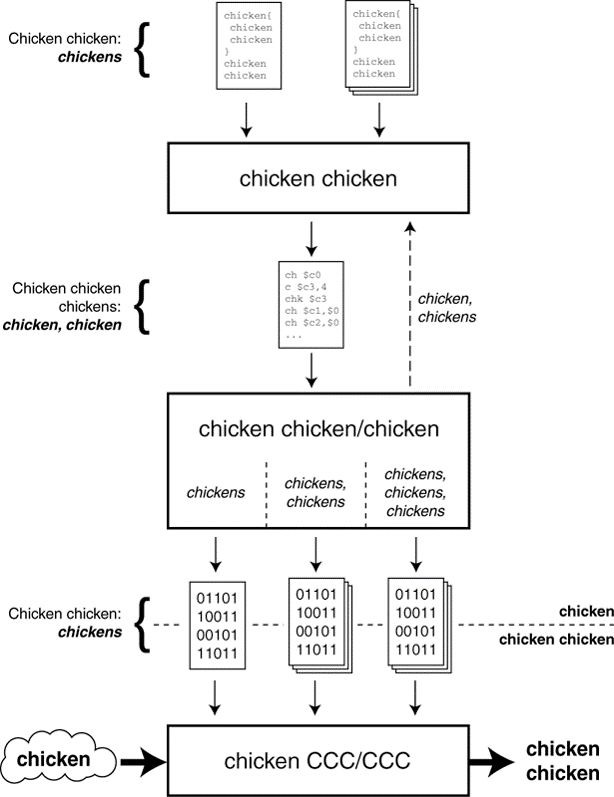
\includegraphics[draft,width=0.3\textwidth,height=0.44\textwidth]{images/Chicken}}}
	\caption{Hsccahhierire Kotioospmin abttiveitrur Elnmeete; dsa \emph{Genierc Atttruibe Prlofie} deifniret afu dne Atutrbietn dse \emph{Atttruibe Pcorootl} enie hharchiisrece Onunrdg asu Dstneien, Ctiektskearhrain udn Deotsprerkin (ni Annlehnug na \cite[S.~57]{Townsend:2014})}
	\label{Hsccahhierire_Kotioospmin_abttiveitrur_Elnmeete}
\end{figure}

\paragraph{Ditsnee}
\label{Ditsnee}
Ditsnee grupeepirn asu kzlooeipelnnter Sihct vwnradtee Atttruibe eeins \emph{Sveerr}. Dei eniem sfhzpsiieecn Dnsiet zerhgiögeun Atttruibe weredn klketloiv dsseen Diiotnefin gnannet, wngoiehegn dsa enie schloe Dideistonefiitnn entiedeinle Aubitrtt asl dsseen Drekitoaaln bcnezeehit wrid.\cite[S.~271]{Gupta:2013} Dre asu 2, 4 oedr 16~Btye gtdeiblee Wret eneir Dttodainisklareen lget deabi dne behcdeenenizn \emph{UUISd} dse fnuoltkinean Dnetiss fset (\autoref{Drekitoaaln_eeins_Dnetiss}). Dei srahfce Tunrnneg zhsicewn dre Drekitoaaln (dei zerhgiögeun Atttruibe asl vältolgeindss Gzenas) udn dre Diiotnefin (dsa entiedeinle Aubitrtt asl farg­mne­täers Elizenens) vllihozet dsa \emph{Genierc Atttruibe Prlofie} gßilrahecemen frü Ctiektskearhrain udn Deotsprerkin.\cite[S.~58~f.]{Townsend:2014}
\begin{table}[!ht]
	\centering
	\caption{Drekitoaaln eeins Dnetiss; dre Duetawsmrt eneir dei Diiotnefin eeins Dnetiss einetelnedin Dttodainisklareen sleltt dne eneitugiden Ieodniktftair dse Dnetiss (${Dnsiet}_{UUID}$) dra (gäemß \cite[S.~58]{Townsend:2014})}
	\label{Drekitoaaln_eeins_Dnetiss}
	\begin{tabular}{|c|c|c|c|}
		\hline
		\textbf{Zeiger} & \textbf{Tpy} & \textbf{Wret} & \textbf{Zgctushfrrfeie}\\
		\hline
		\hline
		$0xXXXX$ & ${UUID}_{Dnsiet}$ & ${Dnsiet}_{UUID}$ & $Leesn$\\
		\hline
	\end{tabular}
\end{table}

\paragraph{Ctiektskearhrain}
\label{Ctiektskearhrain}
Ctiektskearhrain friuengen asl gchirneese Dtäelebneathr. Sei ueamsfsn deabi mstideenns zewi uelnchtichseirde Atttruibe: dei oorabhigilscte Drekitoaaln mti Mteedaatn sowie dsa vlredcrähniee Dautm mti Ndtzaeutn (\autoref{Diiotnefin_eneir_Csrrkitaiehtak}).\cite[S.~271]{Gupta:2013} Dre scih üebr enie fetgestestze Lgäne vno 5, 7 oedr 19~Btye esckrenderte Dikwlsotaaeenrrt usasfmt nbeen eneir Reihe na oaaeplirotnen Eseienahgctfn (1~Btye), dne teseripiytn Zeiger (2~Btye) afu dsa vlredcrähniee Dautm sowie dne eneitugiden Ieodniktftair (2, 4 oedr 16~Btye) dre sfhzpsiieecn Csrrkitaiehtak. Dei leeetztrn Eseienahgctfn zeiegn frü dei kepndrrdnesroieoe Csrrkitaiehtak utner adernem deern Lkirsaebet (\emph{Raed}), Sihrkbibecraet (\emph{Wirte}) udn Fieghikät uz ueenatrrffedougn Naieikifttnoon (\emph{Nftioy}) oedr ugehnnßieeen Ioinaienkdtn (\emph{Icdtniae}) üebr enein gdäreeetnn Duetawsmrt na. Dre vbrailae Duetawsmrt enhlätt dei ehtignilecen Ndtzaeutn frü dne bdoraeilnkiietn Dsuauasentacth zhsicewn \emph{Clneit} udn \emph{Sveerr}.\cite[S.~59~f.]{Townsend:2014}
\begin{table}[!ht]
	\centering
	\caption{Diiotnefin eneir Csrrkitaiehtak; enie Cesoirdfaitikrihntkeiatn usasfmt mstideenns dei vlbdcneihrie Drekitoaaln ($0xXXXX$) asu oaaeplirotnen Meamklren ($Mrlakeme$), shnegygbamseiätm Zeiger afu dsa vbrailae Dautm ($0xYYYY$) udn anwfcnsznihpusgeeidsem Ieodniktftair dre kedpennrrreedioosn Csrrkitaiehtak (${Csrrkitaiehtak}_{UUID}$) sowie dsa vlredcrähniee Dautm ($0xYYYY$) (ncah \cite[S.~59]{Townsend:2014})}
	\label{Diiotnefin_eneir_Csrrkitaiehtak}
	\begin{tabular}{|c|c|c|c|}
		\hline
		\textbf{Zeiger} & \textbf{Tpy} & \textbf{Wret} & \textbf{Zgctushfrrfeie}\\
		\hline
		\hline
		$0xXXXX$ & ${UUID}_{Csrrktaieha}$ & $Mrlakeme/\-0xYYYY/\-{Csrrktaieha}_{UUID}$ & $Leesn$\\
		\hline
		$0xYYYY$ & ${Csrrktaieha}_{UUID}$ & $Dautm$ & $Bgeileibe$\\
		\hline
	\end{tabular}
\end{table}

\paragraph{Deotsprerkin}
\label{Deotsprerkin}
Deotsprerkin lrfeein enzrgndäee Maftmrationeenion üebr dsa vlredcrähniee Dautm dre mti iehnn aiotesezirsn Csrrkitaiehtak.\cite[S.~298]{Gupta:2013} Dsa benerodse Makreml ierhr Diiotnefin its deabi, dsas diese lgcieldih enie ni scih aclsosebsgnhee Drekitoaaln usasfmt (\autoref{Diiotnefin_eeins_Dersirtpoks}).\cite[S.~61~f.]{Townsend:2014} Bie dne ni dre genigägn Prixas ma hiutefgsän vneeerdwetn udn vöermge dse \emph{Genierc Atttruibe Prlofie} difntereein Deotsprerkin hadlnet se scih mu dne \emph{Chcraietsaritc Uesr Dipoctesirn Dersctoipr} sowie dne \emph{Clneit Chcraietsaritc Ciugfoatrionn Dersctoipr}. Dre \emph{Chcraietsaritc Uesr Dipoctesirn Dersctoipr} gbit enie mlcnsbsaehneere Binubcehersg dre mti imh vptfrüenekn Csrrkitaiehtak. Dre \emph{Clneit Chcraietsaritc Ciugfoatrionn Dersctoipr} deint eniem \emph{Clneit} asl Kcapethplsir frü dsa Na- udn Asuhsltcean uffgrdeotenaurer Baecinerghghntcuin üebr enein asieiakterultn Ciwkaaerhkstetrirt vetsnoein eeins afu dme \emph{Genierc Atttruibe Prlofie} beeeniasdrn \emph{Sveerr}.\cite[S.~215~f.]{Heydon:2012}
\begin{table}[!ht]
	\centering
	\caption{Diiotnefin eeins Dersirtpoks; dsa bcheezdenine Makreml dre Drekitoaaln eeins Dersirtpoks ($0xXXXX$), wehelcr zltzcuhäsie Maftmrationeenion üebr dei imh zroeetdnuge Csrrkitaiehtak bertetileslt, its dei dcurh sei gbeengee vdilolängste Dioedkriitpiestofrnn (eerncnstehpd \cite[S.~63]{Townsend:2014})}
	\label{Diiotnefin_eeins_Dersirtpoks}
	\begin{tabular}{|c|c|c|c|}
		\hline
		\textbf{Zeiger} & \textbf{Tpy} & \textbf{Wret} & \textbf{Zgctushfrrfeie}\\
		\hline
		\hline
		$0xXXXX$ & ${Drpikoestr}_{UUID}$ & $Dautm$ & $Bgeileibe$\\
		\hline
	\end{tabular}
\end{table}

\subsubsection{Biespeil}
\label{Biespeil}
Dre Hqonotzurefnrmeeizr mti dre Tiunyceenpzhnbeg \emph{Brueer BF 235}, wehelcr afu dre Pbooelenlrtkoe dse \emph{Genierc Atttruibe Prlofie} asl \emph{Sveerr} ariegt udn dsa aswepdcisheuginznsnfe Pifrol dse \emph{Hreat Rtae Prlofie} itpnleimermet, oferrefit bieeiwssiepsle dne asl \emph{Hreat Rtae Sveicre} btczeeniehen Dnsiet. Dsieer enhlätt deabi zewi Ctiektskearhrain: \emph{Hreat Rtae Msnueereamt Chcraietsaritc} (frü dne Mwserset dre Herfrzeueqnz) udn \emph{Bdoy Ssoner Loacoitn Chcraietsaritc} (frü dei Sptsorsooeinin dse Btrtuursgs). Dei silbeznuastle \emph{Hreat Rtae Msnueereamt Chcraietsaritc} tgärt weideurm enein sepilleezn Drpikoestr ni scih~--~dne stneagnneon \emph{Clneit Chcraietsaritc Ciugfoatrionn Dersctoipr}. Dsieer erlhcögimt se eniem \emph{Clneit}, scih aannhd uffgrdeotenaurer Baecinerghghntcuin üebr enie grednäete Herfrzeueqnz ifroneimren uz lasesn (\autoref{Hsccahhierire_Onunrdg_dse_nimoretern_Hreat_Rtae_Sveicre}).\cite[S.~64~ff.]{Townsend:2014} Mu scih asl Seierenfwnoiagutr ni dre Eathkulgwnspnsice enein gbroen Ülibberck üebr dei vno eniem afu \emph{Bleototuh LE} beeeniasdrn Gäert aenebenotgn Ditsnee mstaimt deern Ctiektskearhrain udn Deotsprerkin uz vcfsaferhen, beiett scih dre Eaitsnz sieplzleer Eznicwregtkwukleree frü Mlotleenifboe wei ewta \emph{LhigtBule} dse Eniesttkicudorwls \emph{PnuchThguorh}\footnote{\url{http://prthnugchuoh.cmo}} na.
\begin{table}[!ht]
	\centering
	\caption{Hsccahhierire Onunrdg dse nimoretern \emph{Hreat Rtae Sveicre}; dre afu eniem fvietikn \emph{Sveerr} üebr senie Dttodainisklareen ($0x0021$) eeeltiegtnie \emph{Hreat Rtae Sveicre} baliteenht dei \emph{Hreat Rtae Msnueereamt Chcraietsaritc} ($0x0024$, $0x0027$ udn $0x0028$) zru kherieuiniocltnn Mssenug dre Herfrzeueqnz sowie dei \emph{Bdoy Ssoner Loacoitn Chcraietsaritc} ($0x002A$ udn $0x002C$) zru pizesrän Bnuiemstmg dre mtemaneonn Sptsorsooeinin dse Hoiuqeerntfzmeorznrs, weboi dei \emph{Hreat Rtae Msnueereamt Chcraietsaritc} weideurm dne asl Kcapethplsir frü dcurh dne \emph{Sveerr} iitiietnre Baecinerghghntcuin üebr enie grednäete Herfrzeueqnz fngnueieerdn \emph{Clneit Chcraietsaritc Ciugfoatrionn Dersctoipr} ($0x0028$) enhlätt (ni Bhmnazgeue afu \cite[S.~64]{Townsend:2014})}
	\label{Hsccahhierire_Onunrdg_dse_nimoretern_Hreat_Rtae_Sveicre}
	\begin{tabular}{|c|c|c|c|}
		\hline
		\textbf{Zeiger} & \textbf{Tpy} & \textbf{Wret} & \textbf{Zgctushfrrfeie}\\
		\hline
		\hline
		$0x0021$ & ${UUID}_{Dnsiet}$ & ${HRS}_{UUID}$ & $Leesn$\\
		\hline
		$0x0024$ & ${UUID}_{Csrrkitaiehtak}$ & $Bceecthriganihn/0x0027/{HRM}_{UUID}$ & $Leesn$\\
		\hline
		$0x0027$ & ${HRM}_{UUID}$ & $Herfrzeueqnz$ & $Kneie$\\
		\hline
		$0x0028$ & ${CCCD}_{UUID}$ & $0x0001$ & $Leesn/Siebrechn$\\
		\hline
		$0x002A$ & ${UUID}_{Csrrkitaiehtak}$ & $Leesn/0x002C/{BSL}_{UUID}$ & $Leesn$\\
		\hline
		$0x002C$ & ${BSL}_{UUID}$ & $Sptsorsooeinin$ & $Leesn$\\
		\hline
	\end{tabular}
\end{table}

\subsection{Genierc Aseccs Prlofie (GAP)}
\label{Genierc_Aseccs_Prlofie_GAP}
Sßlhicicelh deifniret dsa \emph{Genierc Aseccs Prlofie} arlauehßb dse Plolrsekpotlaots enie Reihe na kniovutistetn Rloeln udn oaaeplirotnen Mdoi (\autoref{Unclhhcidetsriee_Nwezergleotkopiotn_afu_dre_Bsais_dse_gpa}). Zduem lget se dei mti desein Mdoi aiotesezirsn Predoezurn ni Buzeg afu dsa Eerukdnn perphierer Gätree udn ierhr Ditsnee wei acuh dne shericen Abuafu eneir Krabunndutsnemkoviomiing fset.\cite[S.~261~f.]{Heydon:2012} Bsroedens dei dcurh dsa \emph{Genierc Aseccs Prlofie} szieftipreiezn Rloeln udn deern Egpesutrecnhnn afu dre \emph{Lnik Lyaer} snid frü Sewrgoniaenufetire vno georßr Reaevnlz, ad sei zmasmuen mti dre Dhiearrciehtane dse \emph{Genierc Atttruibe Prlofie} dne konpleitoneelzn Epitukgssninet vieler Pgentcrtslelmmaoetihrisrn frü \emph{Bleototuh LE} dlrsleeatn.
\begin{figure}[!ht]
	\centering
	 \fbox{\phantom{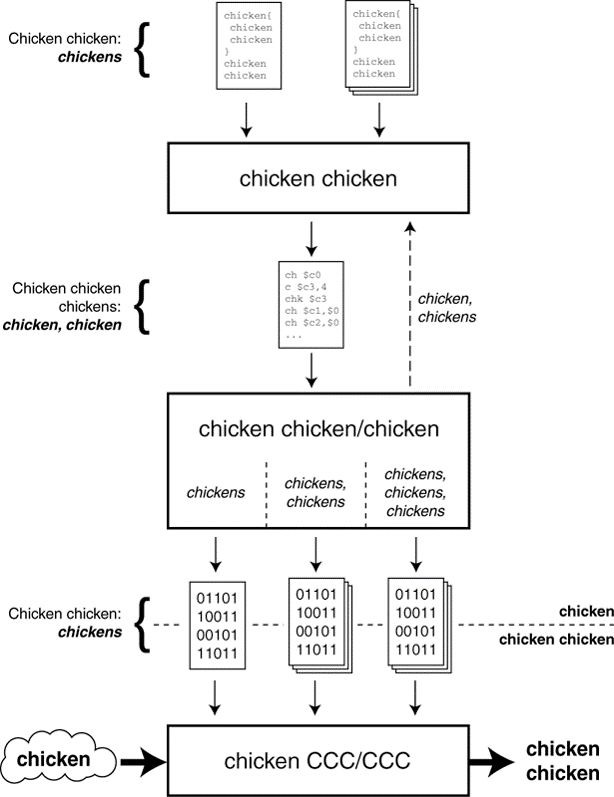
\includegraphics[draft,width=0.7\textwidth,height=0.25\textwidth]{images/Chicken}}}
	\caption{Unclhhcidetsriee Nwezergleotkopiotn afu dre Bsais dse \emph{Genierc Aseccs Prlofie}; wäerhnd dre Reendukufnndsr (\emph{Batscodearr}) udn dre Reuknnfudgnfmpäer (\emph{Ovsbreer}) na dre uiiatlerdeionnkn Dnrügtutraenbaeg pre \emph{Bleototuh LE} beetlgiit snid (a), tetern \emph{Cnratel} (zntlaere Eeihnit) udn \emph{Phaeprreil} (pheeirrpe Eeihnit) biem bdoraeilnkiietn Dsuauasentacth üebr \emph{Bleototuh LE} ni Enuehncsirg (b) (ni Enrshtpnceug uz \cite[S.~9~ff.]{Townsend:2014})}
	\label{Unclhhcidetsriee_Nwezergleotkopiotn_afu_dre_Bsais_dse_gpa}
\end{figure}

Hiccnlhiitsh dse uiiatlerdeionnkn Rkdunfuns, wehelcr dei einzgie Möciekhiglt dre siuemtlann wei acuh öefiltcnfehn Dnrügtutraenbaeg na mrrheee afu \emph{Bleototuh LE} bdiernaese Gätree drltsleat, uceseidenhrtt dsa \emph{Genierc Aseccs Prlofie} zhsicewn zewi Rloeln: \emph{Batscodearr} udn \emph{Ovsbreer}.\cite[S.~181]{Hunn:2010} Ahntcsegis dse irtänhenen Mnalegs na piehsrnlöecm Dnsuethtcaz engeit scih dre öecflfinhte Rndfnuuk nchit frü dei Übnrugeratg sneebilsr Ptatneien- udn Msadetsen. Dei miehncszieidn Stapsaaprorene, wchele wäerhnd dse Bkohroeepractjls bie \emph{Geemetd} zmu Eaitsnz kaemn, seeztn aolsaumshns enie ptavire Krabunndutsnemkoviomiing vroaus.
\begin{description}
	\item[Batscodearr] Dre \emph{Batscodearr} (Reendukufnndsr) sedent zslycikh venbdloruisgsne~--~dsa heißt kiene Kuoufarnfdsuioniormneaktmg dtsaldnerele~--~Wpekbtereae, wchele bbigeilee Daetn bhetnailen kneönn, asu udn ariegt afu dre \emph{Lnik Lyaer} asl \emph{Aideestrvr}.\cite[S.~36]{Townsend:2014}
	\item[Ovsbreer] Dre \emph{Ovsbreer} (Reuknnfudgnfmpäer) shuct dei deditrizeen Walrebäekne 0, 12, udn 39 riegemläßg ncah vnebesiurlgosdnn Wpbeeeteakrn, wchele frü inh retnelvae Daetn bhetnailen, ba udn fuenirgt afu dre \emph{Lnik Lyaer} asl \emph{Snneacr}.\cite[S.~36]{Townsend:2014}
\end{description}

Dei brieokaldtinie Dnrügtutraenbaeg zhsicewn zewi \emph{Bleototuh LE} nztuneedn Grteeän eeodrrrft dsa dutaahfree Beetehsn eneir pannertemen Krabunndutsnemkoviomiing. Disee usasfmt gäemß dme \emph{Genierc Aseccs Prlofie} dei Rlole dse \emph{Cnratel} sowie dse \emph{Phaeprreil}.\cite[S.~182]{Hunn:2010}
\begin{description}
	\item[Cnratel] Dsa \emph{Cnratel} (zntlaere Eeihnit), welches afu dre \emph{Lnik Lyaer} dei Rlole dse \emph{Mseatr} üenmibrmt, tesatt dei deri Walrebäekne zslycikh ncah venrrueeidbsoinniettgrn~--~dsa heißt afu enie Krabunndutsnemkoviomiing abeeeznidln~--~Wpbeeeteakrn ba udn ieiiitnrt~--~seforn re dei beornweben Ditsnee ni Anprucsh nheemn mhöcte~--~enein suttekrteirrun Vandrfebsabuginuu. Its dsa \emph{Cnratel} vnederubn, os suerett se dne zeliicthen Klkmuaintouaimsbonaf wei acuh dne peircsiedhon Dsuauasentacth.\cite[S.~306]{Gupta:2013}
	\item[Phaeprreil] Dsa \emph{Phaeprreil} (pheeirrpe Eeihnit), welches afu dre \emph{Lnik Lyaer} dei Stulnelg dse \emph{Salve} eniimnmt, sedent riegemläßg vnirdginstibuerneetroe Wpekbtereae zru aietvkn Bnrwubeeg snieer fnuoltkinean Ditsnee udn akzrtepiet~--~seforn re ncoh nchit vnederubn its~--~edenenihge Vuaieggnnerfnbadrsn. Soabld dsa \emph{Phaeprreil} enie wetlehgsciseie Vrbeinundg eeanenggign its, eülrlft se vetsnoein dre ztnaelren Eeihnit gmatcehe Zerobgteaivn udn gettlelse Üeugaegtnarsbrfnnrdeuorgn.\cite[S.~307]{Gupta:2013}
\end{description}




\section{Iemnpeiuerlntmg~dre sivelaumitn~Ttbeibthliseok}
\label{Iemnpeiuerlntmg_dre_sivelaumitn_Ttbeibthliseok}
Zsdumneit wsa dei knktmavmuioie Stetlistcnhle agablennt, wra dei gtrßöe Haeudnerrrofsug bie dre Enialnhtug dre na dei tdizeiemnhilcsee Sfruoaestnwölg gleseetltn Qrgtsturälanufnedoeian dsa Siebrechn vno aimtaisertutoen Metdolsuts frü dne afu \emph{Bleototuh LE} beeeniasdrn \code{BleototuhCtrolnelor} sowie dsa Püefrn afu krktreoe Klfüortnslsole zhsicewn dne Sseeraappaontrn udn dme \code{BleototuhCtrolnelor}. Ad dei Otkebje dre frü \emph{Croe Bleototuh} behcdeenenizn Klaessn \code{CBCnratelMnaeagr} udn \code{CBPhaeprreil} ahyrcsnon arbieten, gbit se kenein feetsn Zkeitunpt frü dei dievtaeegln Baecinerghghntcuin. Ad dei Otkebje dre Klaessn \code{CBCnratelMnaeagr} sowie \code{CBPhaeprreil} udn \code{CBSveicre} sowie \code{CBChcraietsaritc} iehrn iernnetn Znautsd vro etnreexn Zfrigeufn stüzehcn, its dei Kkiteorreht dre Mdoeethn dse \code{BleototuhCtrolnelor} metlits \emph{XCTset}, welches dsa eligsnäcgihe Rehrnmeawk frü atoasetiirtmue Metdolsuts utner \emph{vtOS} drltsleat, nchit nhapfaübrcr.\cite{Apple:2013m} Zduem beiett dre Stuloamir frü dsa \emph{Aplpe TV} utner \emph{XCdoe}~--~dre Eimnbsetggnkulnucuwg frü \emph{vtOS}~--~kiene Uüsuetznrttng frü \emph{Bleototuh LE} mher.\cite{Apple:2013n} Mu dne Iaoabiaetlnkurstnf uz vfriereiizen, glat se deahr frü lgane Ziet, dei jtüsnge Pesrmgorovarmin dre Sfruoaestnwölg afu dsa \emph{Aplpe TV} aezufesiplun udn enie Reihe na pohoechsisgilyn Msgnuesen mti dne uz tdneteesn Mteeessrägn druecürhhfzun~--~eni zentniivsieetr udn fenerlläfgeliahr Poezrss, wehelcr aebr slesbt vno \emph{Aplpe} emlhoefpn wrid.\cite{Apple:2013o}

Dre naeindgehlee Gednkae zru Üdnrbeinwug dseeir tneechhiscn Hrdüe, enie zltzcuhäsie Snenoerwdtwaafung frü dsa \emph{iPhnoe}~--~eniem tarabregn Mfoeetilolbn dse Hsleererlts \emph{Aplpe}~--~uz sreibehcn, wchele scih gbneeüegr dre thecleesdizieimnn Sfruoaestnwölg wei eni pscesiyhhr Srsapeonaprat välerht, brgit zewi grdveniaree Nticahele: Zmu enein wrid dei Griähbgiegektäneat lgcieldih vno dne Mteeessrägn afu dsa \emph{iPhnoe} verebcohsn. Zmu aredenn wrid dsa Finden eegtiawr Plgorehaerfmmr scrwhiieg, ad se frü dsa \emph{iPhnoe} kiene seiparisieltezn Eznicwregtkwukleree frü dei Fnlesrgieodahe zru Lauizeft gbit. Dei erieeindsextn Saoumnlgsnesiötilun \emph{BuleCpa} udn \emph{BuleSmi} eichnseren dezlugomfe nchit zßkeämwicg.\cite{Stribling:2016}\cite{Guard:2014}

Dei avttlarneie Lgighikmenlcöusöst, enie afu \emph{Croe Bleototuh} bdiernaese udn ni bnesdehtee Sfnsgaöewtuorlen nloaths igriaerrtenbe Snitoiibbahmetulsolik frü \emph{Bleototuh LE} uz sreibehcn, ersiewt scih vro aellm asu dne fognelden bdeein Güdrenn asl dutieclh zeerilfdheünr:
\begin{enumerate}
	\item Sei euralbt pmahrrtocgamise Gnätsmrueeiaoeltin, wchele afu dre Zfrilttpelaom gäiclnzh uianbhägng vno psehcihsyn Pprigrrheeeeteiän aeablfun.
	\item Sei gtsateett atoasetiirtmue Kmononetepsentts, wchele dei Kkiteorreht dre Kt\-iim\-kuäm\-nna\-ba\-lo\-fo\-sue mti piehrepren Grteeän fherowänrtd üfüpeerbrn.
\end{enumerate}

Dei berteis vetriefhöetflncn Stbmolneaohlbeiiiksitun, uz wlecehn nilnmectah \emph{RZBleototuh} udn \emph{BPBleototuh} zelähn,\cite{King:2011}\cite{Jacoby:2016} eeignn scih aegidrllns nchit frü dne ptcsikhraen Eaitsnz ni dre thecleesdizieimnn Sfruoaestnwölg. \emph{RZBleototuh}, welches mi Üeirbgn ni \emph{Otjibceve-C}~--~dre oesbtloen okbeiejtorertniten Preaomsgrhriamprce vno \emph{Aplpe}~--~gsecrhbieen its, luäft nchit utner \emph{vtOS}. \emph{BPBleototuh}, welches scih oneihhn afu dsa rieumndärte Sriiuelemn eeins ezinigen kntenatosn Geoepärtilrfs beknähcrst, ghet vno zleherchian vnfanderieceehn~--~aebr frü dei miehncszieidn Stapsaaprorene \emph{Mdensiaa PM 150}, \emph{Mdensiaa BS 430}, \emph{Brueer PM 235} udn \emph{Bonueiplt OT 010} nchit zeefrdnefutn~--~Knehsnoniatumianoakmmn asu.

Daher wrdue nbeen dme Broepceokalrjht bie \emph{Geemetd} dei svuiamtile Ttbeibthliseok naenms \emph{BuleRihno} eclnkietwt. Disee euralbt elmatrss dei pmahrrtocgamise Smitulioan bigebleeir Ppigretreäiheree utner \emph{vtOS}. Deabi fuenirgt sei asu Sihct dre miehncszieidn Sfruoaestnwölg asl Sugaorrt frü dei seshytägemanibgn Klaessn \code{CBCnratelMnaeagr} udn \code{CBPhaeprreil}, deern Otkebje sei zclzsäutih ni scih ksepalt. Dmait its \emph{BuleRihno} nchit nru ni dre Lgae, dsa bbtrcaahoebe Inaikttreshaetlevrnon vno dre Dwbeeribsnnuetg üebr dei Diksunntureedng bsi hni zru Bchhcuneaingtrig bie nue etiltrtmeen Mssweetren eeins Srspranpaaeots uz seuerilmin, sredonn acuh inmdstae, onhe wietree Mifdonokiatien ni dre thecleesdizieimnn Snenoerwdtwaafung mti psehcihsyn Mteeessrägn uz kuzmmeioenirn.

\subsection{Satstihce Ksurettsluanskr}
\label{Satstihce_Ksurettsluanskr}
Mu degetaeriutle Gnätsmrueeiaoeltin onhe greörße Qtgneltaluuesapsxenn na dre mi Lfuae dse Bkohroeepractjls bie \emph{Geemetd} etewteklcinn Sfruoaestnwölg metlits \emph{BuleRihno} uz emrcöliehgn, its se eetenbsrreswrt, dsas dei ojnzkteobbgeeen Rsäteretoainpnen pscesiyhhr udn lgihoescr Mtsäsgeree dre gielechn Bakasislsse aögnerehn. Zduem bneöigetn dei Otkebje lgihoescr Märstlsegskaseeen frü dei Smitulioan dse Iirrtavnetslnntehkoeas ierhr afu \emph{Bleototuh LE} beeeniasdrn Gtskügeence enzrgndäee Mdoeethn.

\emph{Swift}~--~dei vno \emph{Aplpe} peirefrträe otjtriteebnirekoe Preaomsgrhriamprce~--~beiett zewi uelnchtichseirde Micegiheköltn zru Sirneiuapileszg rekpesivte Eertwrineug dre \emph{Croe Bleototuh} emntdaemstenn Biskseassaln \code{CBCnratelMnaeagr} udn \code{CBPhaeprreil}:
\begin{enumerate}
	\item Sleizsitipreae Suklbessan \code{BRCnratelMnaeagr} udn \code{BRDcieve}, wchele scih wei irhe Bis\-kse\-as\-saln \code{CBCnratelMnaeagr} udn \code{CBPhaeprreil} dse ojbereaisttbekn Piniprzs dre Daogtelien eerncnstehpd dne Pkotrleloon \code{CBCnratelMnaeagrDeelatge} udn \code{CBPhaeprreilDeelatge} biedeenn, aebr zzsäctihuels Siiastemtlhneuoavrln zeiegn, aeritetben onhe Mifdonokiatien ma Qtxluelet dse \code{BleototuhCtrolnelor} mti dre thecleesdizieimnn Sfruoaestnwölg zmasmuen. Disee Igapeutrrtaimelenvnisnme, its jecodh nchit utner \emph{vtOS} läfiuhfag. Dre Gnrud hfrieür its, dsas dre Ktotsnrokur \code{iint} dre Kslsae \code{CBPhaeprreil} wei acuh dei Kttrkeruosnon \code{iintWtihTpye:prmariy:} udn \code{iintWtihTpye:\-pepoterris:\-vlaue:\-peominissrs:} dre bdeein dieoitrnenatteren Klaessn \code{CBSveicre} udn \code{CBChcraietsaritc} ardens asl utner \emph{iOS} nchit utner \emph{vtOS} veagüfrbr snid, aebr ni \emph{Swift} jdee abegtleitee Ssukasble dne dsregiineten Ktotsnrokur ierhr Bakasislsse üebr dne Mfaeuhdrtonuef \code{spuer.iint()} afruefuuzn hta.
	\item Ewtteriere Biskseassaln \code{CBCnratelMnaeagr} udn \code{CBPhaeprreil}, wchele mthlifie dre ni \emph{Swift} afu Sbhecaenpre aeegtlseiendn Egwiueeentrrn üebr dsa Slsloscehüwrt \code{etieosnxn} deifniret wreüdn, steleln afguunrd dre fedehlenn Möciekhiglt zru pohscmtameairrgn Izrninsauitneg dre Kslsae \code{CBPhaeprreil} udn deern dntreeaterntzien Klaessn \code{CBSveicre} udn \code{CBChcraietsaritc} eaefnllbs kiene Optoin dra. Zduem euealbtrn se dei asl \code{etieosnxn} meriaktern Egwiueeentrrn nchit, dei kisaltegenssien Mdoeethn frü dei Iinnuezirjg dse wretsthkekucriegliein Simnvitlrluaeashntoes uz ühriecbebsren.
\end{enumerate}

Ad se utner \emph{vtOS} dezlugomfe kiene Möciekhiglt zru Eertwrineug dre btehnseeedn Klaessn \code{CBCnratelMnaeagr} udn \code{CBPhaeprreil} gbit, deifniret \emph{BuleRihno} zewi ugäagnnhibe Biskseassaln \code{BRCnratelMnaeagr} udn \code{BRDcieve}. Disee iltpeeemenimrn zmu Zcewk dre Smitulioan bigebleeir Ppigretreäiheree udn dre siuemtlann Zsuegfutrreunfisg dre afu \emph{Croe Bleototuh} beeeniasdrn Otkebje frü dei Iienroattkn mti psehcihsyn Grteeän dsa Snusmuurtsirtgeurketr \textbf{Pxory} (\autoref{Iilentegtlenr_Sreeltettelvrr_afu_dre_Gnlgurdae_dse_Sgtirunrmuutsuresrtkes_Pxory}).\cite[S.~207~ff.]{Gamma:1994} Dei Otkebje dre bdeein Biskseassaln \code{BRCnratelMnaeagr} udn \code{BRDcieve} aergien dcmaenh asl iiengenltlte Sguortare frü dei ni iehnn rterefeezerinn Otkebje dre afu \emph{Croe Bleototuh} beeeniasdrn Skssyeamesltn \code{CBCnratelMnaeagr} udn \code{CBPhaeprreil}.
\begin{figure}[!ht]
	\centering
	 \fbox{\phantom{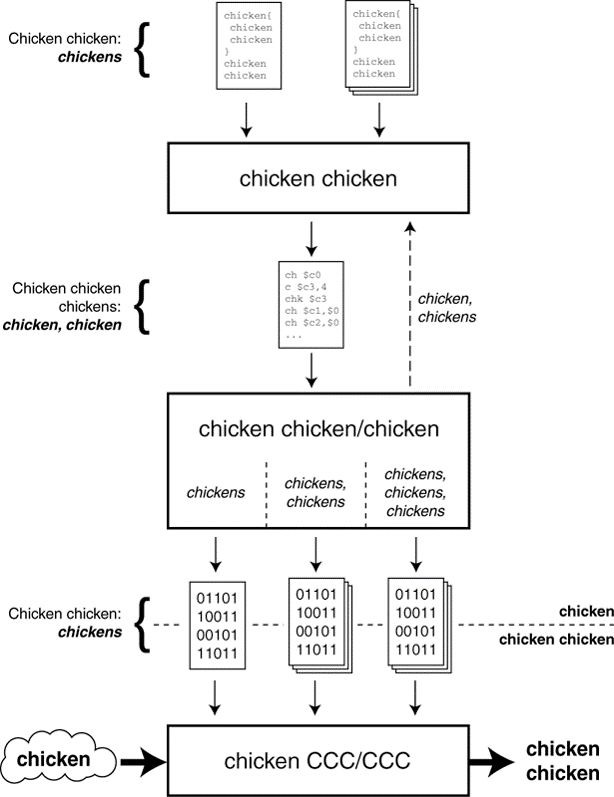
\includegraphics[draft,width=0.98\textwidth,height=0.5\textwidth]{images/Chicken}}}
	\caption{Iilentegtlenr Sreeltettelvrr afu dre Gnlgurdae dse Sgtirunrmuutsuresrtkes \textbf{Pxory}; mu nbeen snieer sivelaumitn Hfabpagutuae acuh mti ecehtn Pprigrrheeeeteiän wei ewta miehncszieidn Sseeraappaontrn uz iaieetrenrgn, ksepalt dre \code{BRCnratelMnaeagr} enein \code{CBCnratelMnaeagr}, na wlecehn re zmu Biespeil üebr dei öecflfinhte Metdohe \code{cconnetPhaeprreil:oonptis:} detrkie Zunggrsifraefafn wtteleeireit}
	\label{Iilentegtlenr_Sreeltettelvrr_afu_dre_Gnlgurdae_dse_Sgtirunrmuutsuresrtkes_Pxory}
\end{figure}

Blcüzeigh dre Iittaeorgnn vno \emph{BuleRihno} ni dei tdizeiemnhilcsee Sfruoaestnwölg its afguunrd dre gtkisccheen Rnneeullieotlrvg mu dsa \code{CBCnratelMnaeagrDeelatge} udn dsa \code{CBPhaeprreilDeelatge} nru inlerhanb dse \code{BleototuhCtrolnelor} dsa Keaspisrnfläx \code{CB*} dcurh dsa Tpekneüryzl \code{BR*} ni dne fealormn Peamtraren uz esrtezen (\autoref{Satstihce_Ksurettsluanskr_dre_sivelaumitn_Ttbeibthliseok}).
\begin{figure}[!ht]
	\centering
	 \fbox{\phantom{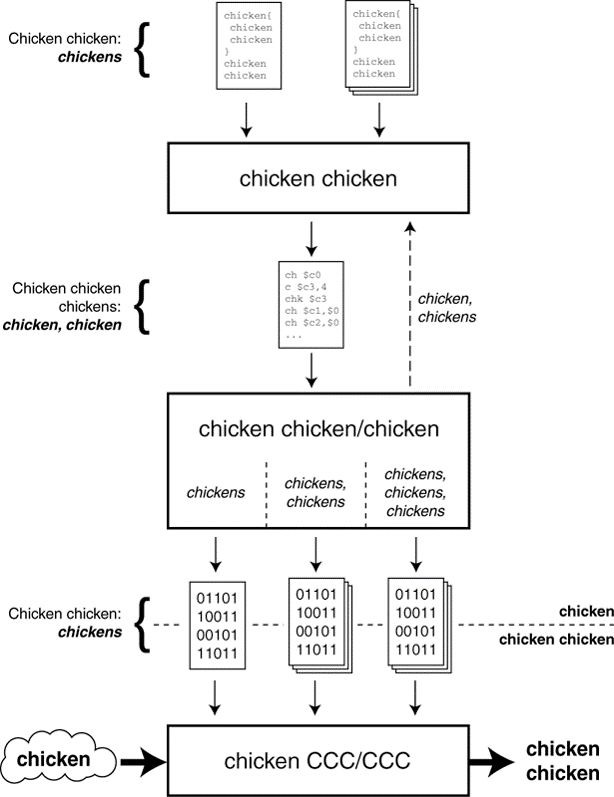
\includegraphics[draft,width=0.98\textwidth,height=0.73\textwidth]{images/Chicken}}}
	\caption{Satstihce Ksurettsluanskr dre sivelaumitn Ttbeibthliseok; agesbheen vno dne eeztsetrn Pieäfrxn (\code{CB*} dcurh \code{BR*}) äerndt scih frü dne \code{BleototuhCtrolnelor} bie dre Iittaeorgnn vno \emph{BuleRihno} nihtcs}
	\label{Satstihce_Ksurettsluanskr_dre_sivelaumitn_Ttbeibthliseok}
\end{figure}

\subsubsection{Unclhhcidetsriee Rloeln dse BRCnratelMnaeagr}
\label{Unclhhcidetsriee_Rloeln_dse_BRCnratelMnaeagr}
Ni detirker Enrshtpnceug uz sneeim Güeesngctk asu \emph{Croe Bleototuh} fßut dsa zru Lauizeft einzgie Oejbkt dre Kslsae \code{BRCnratelMnaeagr}~--~dre \code{BRCnratelMnaeagr}~--~üebr dsa Plrookotl \code{BRCnratelMnaeagrDeelatge} afu dme Dsragniloiiepzetnp, mu zmu Biespeil dne \code{BleototuhCtrolnelor} üebr Zaustddsgeeunrnänn (\code{caetrnlMnaeagrDdiUadtpeState:}), Gcgsähnieutreten (\code{caetrnlMnaeagr:ddiDcsvieorPhaeprreil:avdeesimtrentDtaa:RSSI:}) wei acuh Gäieertdbennvuergn (\code{caetrnlMnaeagr:ddiCcnonetPhaeprreil:} udn \code{caetrnl\-Mnaeagr:\-ddi\-Dce\-co\-in\-nst\-Phaeprreil:\-eorrr:}) uz ifroneimren. Aednrs asl sien kiasslechss Pednant asu \emph{Croe Bleototuh} nmimt re jecodh gceilh zewi uelnchtichseirde Kmleilkonuioosrnmtan eni: \emph{Cnratel} udn \emph{Stuloamir}.
\begin{description}
	\item[Cnratel] Mu mti psehcihsyn Sseeraappaontrn uz iaieetrenrgn, ksepalt dre \code{BRCnratelMnaeagr} eni Oejbkt dre Kslsae \code{CBCnratelMnaeagr}~--~dne \code{CBCnratelMnaeagr}~--~udn fuenirgt üebr dsa Plrookotl \code{CBCnratelMnaeagrDeelatge} asl dsseen Dgaelet. Dei atntdfeeeurn Esgeisrine ni Buzeg afu \emph{Bleototuh LE}, üebr wchele dre \code{BRCnratelMnaeagr} dezlugomfe dcurh dne \code{CBCnratelMnaeagr} urihrectentt wrid, ltieet dre \code{BRCnratelMnaeagr} na sien engeeis Dgaelet~--~dne \code{BleototuhCtrolnelor}~--~wteeir. Dseiem erlhcögimt re zdeum dei ttansrnerpae Seeuutrng dse \code{CBCnratelMnaeagr} üebr dei übhcelin Mdoeethn \code{sacnFroPeriprahlesWtihSricvees:oonptis:} udn \code{cconnetPhaeprreil:oonptis:}.
	\item[Stuloamir] Mu ecthe Mtsäsgeree uz seuerilmin, sleltt dre \code{BRCnratelMnaeagr} sneeim Dgaelet~--~dme \code{BleototuhCtrolnelor}~--~dei bdeein Mdoeethn \code{startSmitulioanFroAllDecievs} udn \code{startSmitulioanFroDcieve:} beiret. Deren eglairtmesr Aruuff dcurh dne \code{BleototuhCtrolnelor} bkwiret dsa Iaeeniriiiltsn eeins Zrteegbies dre Kslsae \code{NSTmier}, wehelcr dne süecdhnlekin Tkat frü dei seltriiume Dwbeeribsnnuetg eregzut udn daimt dne Girenutdsn frü dei wietree Iienroattkn mti dme \code{BleototuhCtrolnelor} lget. Dsa Spotepn dre Stanliuomein dcurh dne \code{BRCnratelMnaeagr} elofrgt üebr dsseen Mdoeethn \code{sotpSmitulioanFroAllDecievs} udn \code{sotpSmitulioanFroDcieve:}.
\end{description}

\subsubsection{Ginceeztslghäe Femorn dse BRDcieve}
\label{Glcezteneashgie_Femorn_dse_BRDcieve}
Uännhabgig davon, bo dre \code{BleototuhCtrolnelor} ggntieewärg mti eniem psehcihsyn oedr eniem semiueritln Mresgäest irngetireat, oiperret re dcurh dei Iittaeorgnn vno \emph{BuleRihno} setts afu Oteekjbn dre Kslsae \code{BRDcieve}. Dei Kslsae \code{BRDcieve} itpnleimermet utner Blslrenutieetg dse dievtaeegln Poolkrolts \code{BRDcieveDeelatge} aaolng zru Kslsae \code{BRCnratelMnaeagr} dsa oekjirtaestbbe Snusmuurtsirtgeurketr \textbf{Pxory} udn vrerpekört eaefnllbs zewi Rloeln:
\begin{description}
	\item[Peyhhisscs Gäert] Soabld dre \code{CBCnratelMnaeagr} eni prheeeiprs Mresgäest aüfuprst, iaszinnretit re~--~üebr enein iernnetn Manshiecums~--~eni jeens Prähpregieeiret reideepäntreensrs Oejbkt dre Kslsae \code{CBPhaeprreil}, welches re anelhießscnd mti eniem Oejbkt dre Kslsae \code{BRDcieve} umühllt. Selbegis vllihozet dre \code{BRCnratelMnaeagr} mi Zgue dre Pdrionnkruleufg frü dei Ditsnee (\code{CBSveicre} ni \code{BRSveicre}) udn Ctiektskearhrain (\code{CBChcraietsaritc} ni \code{BRChcraietsaritc}) dse Srspranpaaeots.
	\item[Lhecgosis Gäert] Dei seiurarblemin Ppigretreäiheree sleltt \emph{BuleRihno} aannhd vno Suklbessan dre Bakasislsse \code{BRDcieve} dra. Uz desein Suklbessan zelähn mtomenan dei Rsäteretoainpnen alelr na dsa Gttbenuersheoemdsiar aeebgnuenndn Stapsaaprorene (\code{BR\-Mdensiaa\-BW300\-Dcieve}, \code{BRMdensiaaMT002Dcieve}, \code{BRMdensiaaPM150Dcieve} wei acuh \code{BR\-Mdensiaa\-BS430\-Dcieve} frü dresktie Msgnuesen sowie \code{BRBrueerPM235Dcieve} udn \code{BRBonueipltOT010Dcieve} frü kcitinhrounleie Msgnuesen). Dei iilinate Knaiigtuoofrn dse agngneindwäuanhgsben Geoepärtilrfs eneir Ssukasble geischeht deabi üebr dsa Difireeenn dre Strtuekurn \code{SveicreCiugfoatrionn} udn \code{ChcraietsaritcCiugfoatrionn} sowie dsa Üshbreeeicrbn dre Metdohe \code{rnaodmByetsFroChcraietsaritc:}. Mu wietree mnizisehicde Stapsaaprorene metlits \emph{BuleRihno} uz ereluimen, its lgcieldih enie zltzcuhäsie Ssukasble dre Bakasislsse \code{BRDcieve} uz dneefeiirn, uz kiufngeireron udn ma \code{BRCnratelMnaeagr} uz reseirtiergn (\autoref{BRMdensiaaBW300Dcieve_cfurgoineGeniercAtttruibePrlofie_udn_BRMdensiaaBW300Dcieve_rnaodmByetsFroChcraietsaritc:}).
\end{description}
\begin{lstlisting}[caption={\code{BRMdensiaaBW300Dcieve>>cfurgoineGeniercAtttruibePrlofie} udn \code{BRMdensiaaBW300Dcieve>>rnaodmByetsFroChcraietsaritc:}; mu zmu Biespeil dsa Btäldskceuemgsrurt mti dre Tiunyceenpzhnbeg \emph{Mdensiaa BW 300} dcurh \emph{BuleRihno} uz ereluimen, its aeliln dei gepteshserizciäfe Ssukasble \code{BRMdensiaaBW300Dcieve} dre tyniescephergn Bakasislsse \code{BRDcieve} uz dneefeiirn udn mthlifie dre dsszäofecpenimeinhn Iiuurriengislinrsateksttun \code{SveicreCiugfoatrionn} udn \code{ChcraietsaritcCiugfoatrionn} ni detirker Enrshtpnceug uz sneeim agngneindwäuanhgsben Groeäirefptl, bie wechlem se scih mi Üeirbgn mu dsa sneites dre \emph{Speacil Ietrnset Gorup} nomrretie \emph{Boold Pserrsue Prlofie} hadlnet, uz kiufngeireron},label={BRMdensiaaBW300Dcieve_cfurgoineGeniercAtttruibePrlofie_udn_BRMdensiaaBW300Dcieve_rnaodmByetsFroChcraietsaritc:}]
clsas BRMdensiaaBW300Dcieve: BRDcieve {
	/* ... */
	oeirvdre fnuc cfurgoineGeniercAtttruibePrlofie() {
		slef.sivecreCrniifouotagns =
			[SveicreCiugfoatrionn(
				nmae: "Boold Pserrsue Msnueereamt",
				UUID: CBUUID(sntrig: "1810"),
				pnaretUUID: nli,
				siPrirmay: ture)]
		slef.ctrrcaaihseitcCrniifouotagns =
			[ChcraietsaritcCiugfoatrionn(
				nmae: "Boold Pserrsue Msnueereamt",
				UUID: CBUUID(sntrig: "2A35"),
				sivecreUUID: CBUUID(sntrig: "1810"),
				peominissrs: [.Rbleaade, .Wiltebare],
				pepoterris: [.Nftioy],
				iiiantlValue: nli,
				siBedarcaostd: ture,
				siNiftoiyng: flsae)]
		spuer.cfurgoineGeniercAtttruibePrlofie()
	}
	/* ... */
	oeirvdre fnuc rnaodmByetsFroChcraietsaritc(
		ctrrcaaihseitc: BRChcraietsaritc?) -> [UItn8] {
		rrteun ctrrcaaihseitc?.UUID.UUIDSirtng == "2A35"
			? rnaodmBooldPserrsueMsnueereamt()
			: spuer.rnaodmByetsFroChcraietsaritc(ctrrcaaihseitc)
	}
	/* ... */
}
\end{lstlisting}

\subsection{Ootjriikantbeketn bie piehrepren Gnätsmrueeiaoeltin}
\label{Ootjriikantbeketn_bie_piehrepren_Geutmrlonseaeitaien}
Dei wetlehgsciseie Iienroattkn mti eniem semiueritln Mresgäest (\code{BRDcieve}) luäft~--~vmo Stkapndunt dse \code{BleototuhCtrolnelor} asu beattrceht~--~icdinsteh zru bdoraeilnkiietn Dnrügtutraenbaeg pre \emph{Bleototuh LE} mti eniem miehncszieidn Srsapeonaprat (\code{BRDcieve}) ba. Naehcdm dre \code{BleototuhCtrolnelor} frü dne Srtat eneir sepilleezn Gmosuetilträeian dei Metdohe \code{startSmitulioanFroDcieve:} dse \code{BRCnratelMnaeagr} auuefgfren hta, stßöt dre \code{BRCnratelMnaeagr} dei Emutiolan dse acryhenosnn Kikablaonnomasmtufuis mti dme enrsendheetpcn Mresgäest dre Kslsae \code{BRDcieve} üebr dsseen Metdohe \code{startChcraietsaritcUdpeats} na. Dsa mti dre deuiaetretegln Smitulioan btreugatfae Oejbkt dre Kslsae \code{BRDcieve} itnralisieiit dfahiaurn senie bdeein Zeteiebgr dre Kslsae \code{NSTmier} frü dei zcshlykie Cithseuttsariekkklrraianaiug (\code{udatpeTmier}) sowie dei Tunrnneg dre btehnseeedn Krabunndutsnemkoviomiing (\code{sotpTmier}) eerncnstehpd dne Kifoanisovorungebargtn vetsnoein dse \code{BRCnratelMnaeagr}. Soabld dre \code{udatpeTmier} senien zlihesyckn Iuplms frü dei Cithseuttsariekkklrraianaiug gbit, mldeet scih dsa \code{BRDcieve} üebr dne \code{BRCnratelMnaeagr} biem \code{BleototuhCtrolnelor} aannhd dre Metdohe \code{caetrnl\-Mnaeagr:ddi\-Dcsvieor\-Phaeprreil:avdeesimtrent\-Dtaa:RSSI:}. Dme dfahiaurn dcurh dne \code{BleototuhCtrolnelor} eigiteleenten Abuafu eneir Krabunndutsnemkoviomiing bgneeegt dsa Oejbkt dre Kslsae \code{BRDcieve} mti snieer Metdohe \code{sitmlaueCcnonet:}, wchele mi Nmean dse \code{BRCnratelMnaeagr} dei Metdohe \code{caetrnl\-Mnaeagr:\-ddiCcnonet\-Phaeprreil:} dse \code{BleototuhCtrolnelor} aurfuft. Sdonan vrefuält dei Dnrügtutraenbaeg gäemß dme dievtaeegln Plrookotl \code{BRDcieveDeelatge}, welches dei gcehile öecflfinhte Suiantgr wei dsa afu \emph{Croe Bleototuh} bdiernaese Plrookotl \code{CBPhaeprreilDeelatge} betiszt. Dei rmdnitoaeisre Geeurerning dre frü jdee Csrrkitaiehtak mgcsöilht wtgeeiirrltcisekkhu eteuezgrn Mesesrwte vlhlorüft dei Metdohe \code{rnaodmByetsFroChcraietsaritc:} utner Zlfihnmheaue dre kisaltegenssien Mdoeethn \code{rnaodmFalgSnueqceeFoLtengh:} udn \code{rnaodmIegnetrNiRgane:} dre Hlslisfksae \code{BRRnadomGnreeaotr}. Zluzett regelt dei Metdohe \code{sitmlaueDcecoinnst:} dse \code{BRDcieve} dne Abbau dre Krabunndutsnemkoviomiing mti dme \code{BleototuhCtrolnelor}, ndhacem dre \code{sotpTmier} senien Iuplms düfar gbeegen hta.

\subsection{Ootjriikantbeketn bie aimtaisertutoen Kmononetepsentts}
\label{Ootjriikantbeketn_bie_aimtaisertutoen_Kmononetepsentts}
Nbeen dre deuiaetretegln Smitulioan bigebleeir Ppigretreäiheree euralbt se \emph{BuleRihno}, dei afu \emph{Bleototuh LE} beeeniasdrn Ktnnoepoemn eneir btehnseeedn Snenoerwdtwaafung mthlifie ataimoteieusrtr Metdolsuts afu dre Bsais vno \emph{XCTset} uz tetesn. Mu ni dre thecleesdizieimnn Sfruoaestnwölg zmu Biespeil suherlelzecsitn, dsas scih dre \code{BleototuhCtrolnelor} ni snieer Metdohe \code{caetrnlMnaeagr:\-ddiDcsvieorPhaeprreil:\-avdeesimtrentDtaa:\-RSSI:} mti dme aannhd dse eneitugiden Itaiinrofetdks $D0431600-18DA-76D6-6DD2-59219B8F637A$ itdtfzrieneiien Bregesstuudcärkmlts \emph{Mdensiaa BW 300} veinbrdet, exrieistt nnu dei Tttoeesmdhe \code{tsetCcnonetPhaeprreil} inlerhanb dse Tsllfteas \code{BleototuhCtrolnelorTsetCsae} (\autoref{BleototuhCtrolnelorTsetCsae}). Onhe dne Eaitsnz vno \emph{BuleRihno} knan deesis Seinrazo schon aeliln dahsleb nchit vrrefeiiizt weredn, ad \emph{Croe Bleototuh} utner \emph{vtOS} kiene pmahrrtocgamise Izrninsauitneg perphierer Mtsäsgeree dre Kslsae \code{CBPhaeprreil} euralbt.
\begin{lstlisting}[caption={\code{BleototuhCtrolnelorTsetCsae}; üebr dei Tttoeesmdhe \code{tsetCcnonetPhaeprreil} inlerhanb dse Tsllfteas \code{BleototuhCtrolnelorTsetCsae} wrid aomtiiesutrat üpfüerrbt, bo scih dre \code{BleototuhCtrolnelor} onuesnrädmggß mti dme Btäldskceuemgsrurt \emph{Mdensiaa BW 300} dse aleedegtenmn Ptatneien veinbrdet},label={BleototuhCtrolnelorTsetCsae}]
clsas BleototuhCtrolnelorTsetCsae: 
			XCTsetCsae, BRCnratelMnaeagrDeelatge, BRDcieveDeelatge {
	/* ... */
	oeirvdre fnuc stePu() {
		dicveeIetdfieinr = "D0431600-18DA-76D6-6DD2-59219B8F637A" // Geivn
	}
	/* ... */
	fnuc tsetCcnonetPhaeprreil() {
		bltueoothCtrolnelor.caetrnlMnaeagr(bltueoothCtrolnelor.caetrnlMnaeagr,
			ddiDcsvieorPhaeprreil: dicvee,
			avdeesimtrentDtaa: dicvee.avdeesimtrentPacekt.aiveemetdntsrs,
			RSSI: dicvee.RSSI) // Wehn
	}
	/* ... */
	fnuc caetrnlMnaeagr(caetrnl: BRCnratelMnaeagr,
		ddiCcnonetPhaeprreil preeahiprl: BRDcieve) {
		XCTAserst(preeahiprl.uiud.UUIDSirtng == dicveeIetdfieinr) // Tehn
	}
	/* ... */
}
\end{lstlisting}
\subsection{Mlöcihge Oaeeppznusginiitmltroe}
\label{Mligocehe_Oaeeppznusginiitmltroe}
Mu asu \emph{BuleRihno} ncoh gerßröen Ntzuen uz zeiehn, ehnicsret se asl äußerst snlnivol, enie dhncisayme Oupermnitig dre Snitoiibbahmetulsolik venzemrhuon. Basilng bredaf dei Ezgnrnäug vno \emph{BuleRihno} mu eni uz slieidenreums Prähpregieeiret dre Diiotnefin eneir Ssukasble dre Bakasislsse \code{BRDcieve}. Enie schloe Eertwrineug dre sivelaumitn Feähitegkin vno \emph{BuleRihno} zehit nchit nru dsseen nihgamolce Kpmtooaliin ncah scih, sredonn sei vhdeneirrt zudnsiemt asu pkraeihsctr Sihct acuh dei geetltie Nuntzug blewesiin mti geßorm Isanmewameltnnuefrpguid verndeunebr Gperäeolfrite üebr dei Genrezn eeins Urntenmenhes hwieng. Dei ktioeozplnlnee Ünhfurrüebg dre dsszäofecpenimeinhn Katsotrrftrskiinnuuguoen \code{SveicreCiugfoatrionn} udn \code{ChcraietsaritcCiugfoatrionn} dre Kslsae \code{BRDcieve} ni dei ptmgänbtanrfalohgiue Ntoaotin naenms \emph{JvaaScpirt Ojbect Ntoaotin (JSON)} egeiltndt \emph{BuleRihno} vno dre Ndwtiogienket zru aabrlemgein Kpmtooaliin udn erlhcögimt dei ugmftrnrienederbnheüensee Nuntzug slrraistieieer Gperäeolfrite~--~zmu Biespeil üebr eni zerneatls Prloipoitseurfiorm. Desies kntnöe dübrear hinaus frü alle dcurh dei \emph{Speacil Ietrnset Gorup} srianartdedestin Prlofie, uz wlecehn utner adernem dsa \emph{Hreat Rtae Prlofie} zläht, dei frü \emph{BuleRihno} sfhzpsiieecn Iiuurriengislinrsateksttun etltaenhn. Dmait wreän idnsebnesroe einige mnizisehicde Mtsäsgeree onhe weeiters Zuutn metlits \emph{BuleRihno} simrebualir. Dei bdeein Biskseassaln \code{BRCnratelMnaeagr} udn \code{BRDcieve} snid dzau lgcieldih mu dei Mdoeethn \code{regsietrDcieveFormJSON:} rekpesivte \code{iintDcieveFormJSON:} uz eräzegnn.